\begin{frame}{Ideas}

  \vspace{3em}
  \begin{itemize}
    \item Pose selection
    \item Scan--to--map-scan matching (backbone of my PhD)
  \end{itemize}

  \vspace{-3em}
  \begin{figure}\centering
    \resizebox{6cm}{!}{% GNUPLOT: LaTeX picture with Postscript
\begingroup
  \makeatletter
  \providecommand\color[2][]{%
    \GenericError{(gnuplot) \space\space\space\@spaces}{%
      Package color not loaded in conjunction with
      terminal option `colourtext'%
    }{See the gnuplot documentation for explanation.%
    }{Either use 'blacktext' in gnuplot or load the package
      color.sty in LaTeX.}%
    \renewcommand\color[2][]{}%
  }%
  \providecommand\includegraphics[2][]{%
    \GenericError{(gnuplot) \space\space\space\@spaces}{%
      Package graphicx or graphics not loaded%
    }{See the gnuplot documentation for explanation.%
    }{The gnuplot epslatex terminal needs graphicx.sty or graphics.sty.}%
    \renewcommand\includegraphics[2][]{}%
  }%
  \providecommand\rotatebox[2]{#2}%
  \@ifundefined{ifGPcolor}{%
    \newif\ifGPcolor
    \GPcolorfalse
  }{}%
  \@ifundefined{ifGPblacktext}{%
    \newif\ifGPblacktext
    \GPblacktexttrue
  }{}%
  % define a \g@addto@macro without @ in the name:
  \let\gplgaddtomacro\g@addto@macro
  % define empty templates for all commands taking text:
  \gdef\gplbacktext{}%
  \gdef\gplfronttext{}%
  \makeatother
  \ifGPblacktext
    % no textcolor at all
    \def\colorrgb#1{}%
    \def\colorgray#1{}%
  \else
    % gray or color?
    \ifGPcolor
      \def\colorrgb#1{\color[rgb]{#1}}%
      \def\colorgray#1{\color[gray]{#1}}%
      \expandafter\def\csname LTw\endcsname{\color{white}}%
      \expandafter\def\csname LTb\endcsname{\color{black}}%
      \expandafter\def\csname LTa\endcsname{\color{black}}%
      \expandafter\def\csname LT0\endcsname{\color[rgb]{1,0,0}}%
      \expandafter\def\csname LT1\endcsname{\color[rgb]{0,1,0}}%
      \expandafter\def\csname LT2\endcsname{\color[rgb]{0,0,1}}%
      \expandafter\def\csname LT3\endcsname{\color[rgb]{1,0,1}}%
      \expandafter\def\csname LT4\endcsname{\color[rgb]{0,1,1}}%
      \expandafter\def\csname LT5\endcsname{\color[rgb]{1,1,0}}%
      \expandafter\def\csname LT6\endcsname{\color[rgb]{0,0,0}}%
      \expandafter\def\csname LT7\endcsname{\color[rgb]{1,0.3,0}}%
      \expandafter\def\csname LT8\endcsname{\color[rgb]{0.5,0.5,0.5}}%
    \else
      % gray
      \def\colorrgb#1{\color{black}}%
      \def\colorgray#1{\color[gray]{#1}}%
      \expandafter\def\csname LTw\endcsname{\color{white}}%
      \expandafter\def\csname LTb\endcsname{\color{black}}%
      \expandafter\def\csname LTa\endcsname{\color{black}}%
      \expandafter\def\csname LT0\endcsname{\color{black}}%
      \expandafter\def\csname LT1\endcsname{\color{black}}%
      \expandafter\def\csname LT2\endcsname{\color{black}}%
      \expandafter\def\csname LT3\endcsname{\color{black}}%
      \expandafter\def\csname LT4\endcsname{\color{black}}%
      \expandafter\def\csname LT5\endcsname{\color{black}}%
      \expandafter\def\csname LT6\endcsname{\color{black}}%
      \expandafter\def\csname LT7\endcsname{\color{black}}%
      \expandafter\def\csname LT8\endcsname{\color{black}}%
    \fi
  \fi
    \setlength{\unitlength}{0.0500bp}%
    \ifx\gptboxheight\undefined%
      \newlength{\gptboxheight}%
      \newlength{\gptboxwidth}%
      \newsavebox{\gptboxtext}%
    \fi%
    \setlength{\fboxrule}{0.5pt}%
    \setlength{\fboxsep}{1pt}%
\begin{picture}(5000.00,5000.00)%
    \gplgaddtomacro\gplbacktext{%
      \colorrgb{0.15,0.15,0.15}%
      \put(518,1546){\makebox(0,0)[r]{\strut{} $+1.0$}}%
      \colorrgb{0.15,0.15,0.15}%
      \put(518,2198){\makebox(0,0)[r]{\strut{} $+2.0$}}%
      \colorrgb{0.15,0.15,0.15}%
      \put(518,2849){\makebox(0,0)[r]{\strut{} $+3.0$}}%
      \colorrgb{0.15,0.15,0.15}%
      \put(518,3501){\makebox(0,0)[r]{\strut{} $+4.0$}}%
      \colorrgb{0.15,0.15,0.15}%
      \put(650,1226){\makebox(0,0){\strut{} $-1.5$}}%
      \colorrgb{0.15,0.15,0.15}%
      %\put(976,1226){\makebox(0,0){\strut{} $-1$}}%
      \colorrgb{0.15,0.15,0.15}%
      \put(1302,1226){\makebox(0,0){\strut{} $-0.5$}}%
      \colorrgb{0.15,0.15,0.15}%
      %\put(1627,1226){\makebox(0,0){\strut{} $0$}}%
      \colorrgb{0.15,0.15,0.15}%
      \put(1953,1226){\makebox(0,0){\strut{} $+0.5$}}%
      \colorrgb{0.15,0.15,0.15}%
      %\put(2279,1226){\makebox(0,0){\strut{} $1.0$}}%
    }%
    \gplgaddtomacro\gplfronttext{%
      \colorrgb{0.00,0.00,0.00}%
      \put(1464,4000){\makebox(0,0){\strut{} Cartesian space}}%
    }%
    \gplgaddtomacro\gplbacktext{%
      \colorrgb{0.15,0.15,0.15}%
      \put(5200,2171){\makebox(0,0)[r]{\strut{} $-2.0$}}%
      \colorrgb{0.15,0.15,0.15}%
      \put(5200,2533){\makebox(0,0)[r]{\strut{} $-1.0$}}%
      \colorrgb{0.15,0.15,0.15}%
      \put(5200,2895){\makebox(0,0)[r]{\strut{} $0.0$}}%
      \colorrgb{0.15,0.15,0.15}%
      \put(5200,3257){\makebox(0,0)[r]{\strut{} $+1.0$}}%
      \colorrgb{0.15,0.15,0.15}%
      \put(3075,1579){\makebox(0,0){\strut{} $-2.0$}}%
      \colorrgb{0.15,0.15,0.15}%
      %\put(3437,1579){\makebox(0,0){\strut{} $-1.0$}}%
      \colorrgb{0.15,0.15,0.15}%
      \put(3800,1579){\makebox(0,0){\strut{} $0.0$}}%
      \colorrgb{0.15,0.15,0.15}%
      %\put(4162,1579){\makebox(0,0){\strut{} $1.0$}}%
      \colorrgb{0.15,0.15,0.15}%
      \put(4524,1579){\makebox(0,0){\strut{} $+2.0$}}%
    }%
    \gplgaddtomacro\gplfronttext{%
      \colorrgb{0.00,0.00,0.00}%
      \put(3709,3794){\makebox(0,0){\strut{} Measurement space}}%
    }%
    \gplbacktext
    \put(0,0){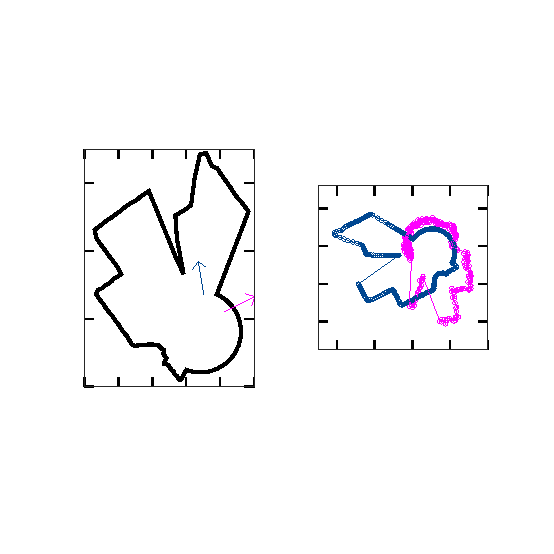
\includegraphics[trim={0 0 0cm 0},clip]{./figures/06/sr5_sm0_init}}%
    \gplfronttext
  \end{picture}%
\endgroup
}
    \vspace{-3em}
    \caption{Left: Unknown LIDAR \textcolor{magenta}{pose $\bm{p}(x,y,\theta)$} and
\textcolor[RGB]{0,71,145}{estimate $\hat{\bm{p}}(\hat{x},\hat{y},\hat{\theta})$}. Right: \textcolor{magenta}{Real $\mathcal{S}_R(\bm{p})$} and
\textcolor[RGB]{0,71,145}{virtual $\mathcal{S}_V(\hat{\bm{p}})$}
scans, in the local coordinate frame of each sensor}
  \end{figure}



\end{frame}
